\uuid{DkOf}
\chapitre{Statistique}
\niveau{L2}
\module{Probabilité et statistique}
\sousChapitre{Tests d'hypothèses, intervalle de confiance}
\titre{Test d'adéquation à une loi}
\theme{statistiques, test du chi-deux, loi de Poisson}
\auteur{Maxime Nguyen}
\datecreate{2022-09-28}
\organisation{AMSCC}
\difficulte{2}
\contenu{
	\texte{ 
		Une enquête a été réalisée auprès de 100 demandeurs d'emploi sur le nombre d'entretiens 
		d'embauche obtenus ces deux derniers mois. Elle donne les résultats suivants :
		
		\begin{center}
			\begin{tabular}{|c|c|c|c|c|c|c|c|}
				\hline 
				\textbf{Nombre d'entretiens :} & 0 & 1 & 2 & 3 & 4 & 5 & 6 et plus \\ 
				\hline 
				\textbf{Effectifs observés :} & 15 & 30 & 27 & 13 & 9 & 5 & 1 \\ 
				\hline 
			\end{tabular} 
		\end{center}
	}
	
	\question{ 
		Peut-on dire que le nombre d'entretiens d'embauche est distribué selon une loi de Poisson ? 
		On utilisera un seuil de significativité $\alpha = 5\%$.
	}
	
	\reponse{
		
		\textbf{Préambule : Rappels sur le test d'adéquation du $\chi^2$}
		
		Le test d'adéquation du $\chi^2$ permet de vérifier si un échantillon suit une loi théorique donnée.
		
		\textbf{Principe :} On compare les effectifs observés $o_i$ avec les effectifs théoriques $e_i$ 
		calculés à partir de la loi supposée. Si les écarts sont trop importants, on rejette l'hypothèse.
		
		\textbf{Conditions d'application :}
		\begin{itemize}
			\item Les observations sont indépendantes
			\item Tous les effectifs théoriques $e_i \geq 5$ (sinon regrouper les classes)
			\item La taille de l'échantillon est suffisante ($n \geq 30$)
		\end{itemize}
		
		\bigskip
		\textbf{ÉTAPE 1 : FORMULATION DES HYPOTHÈSES}
		
		Soit $X$ la variable aléatoire représentant le nombre d'entretiens d'embauche obtenus 
		par un demandeur d'emploi.
		
		\begin{itemize}
			\item \textbf{Hypothèse nulle $H_0$ :} $X$ suit une loi de Poisson de paramètre $\lambda$
			\item \textbf{Hypothèse alternative $H_1$ :} $X$ ne suit pas une loi de Poisson
		\end{itemize}
		
		Il s'agit d'un test bilatéral.
		
		\bigskip
		\textbf{ÉTAPE 2 : ESTIMATION DU PARAMÈTRE $\lambda$}
		
		Sous $H_0$, si $X \sim \mathcal{P}(\lambda)$, alors $\mathbb{E}(X) = \lambda$.
		
		On estime $\lambda$ par la moyenne empirique des observations :
		$$\hat{\lambda} = \bar{x} = \frac{1}{n}\sum_{i} x_i \cdot o_i$$
		
		\textbf{Calcul détaillé :}
		\begin{align*}
			\hat{\lambda} &= \frac{1}{100}(0 \times 15 + 1 \times 30 + 2 \times 27 + 3 \times 13 + 4 \times 9 + 5 \times 5 + 6 \times 1) \\
			&= \frac{1}{100}(0 + 30 + 54 + 39 + 36 + 25 + 6) \\
			&= \frac{190}{100} \\
			&= 1.90
		\end{align*}
		
		On estime donc $\lambda \approx 1.90$.
		
		\bigskip
		\textbf{ÉTAPE 3 : CALCUL DES EFFECTIFS THÉORIQUES}
		
		Pour une loi de Poisson $\mathcal{P}(1.90)$, la probabilité d'obtenir $k$ entretiens est :
		$$P(X = k) = \frac{e^{-1.90} \times (1.90)^k}{k!}$$
		
		Les effectifs théoriques sont : $e_k = n \times P(X = k) = 100 \times P(X = k)$
		
		\textbf{Calculs des probabilités :}
		
		\begin{itemize}
			\item $P(X = 0) = \frac{e^{-1.90} \times (1.90)^0}{0!} = e^{-1.90} \approx 0.1496$
			
			\item $P(X = 1) = \frac{e^{-1.90} \times (1.90)^1}{1!} = 1.90 \times e^{-1.90} \approx 0.2842$
			
			\item $P(X = 2) = \frac{e^{-1.90} \times (1.90)^2}{2!} = \frac{3.61 \times e^{-1.90}}{2} \approx 0.2700$
			
			\item $P(X = 3) = \frac{e^{-1.90} \times (1.90)^3}{3!} = \frac{6.859 \times e^{-1.90}}{6} \approx 0.1710$
			
			\item $P(X = 4) = \frac{e^{-1.90} \times (1.90)^4}{4!} = \frac{13.032 \times e^{-1.90}}{24} \approx 0.0812$
			
			\item $P(X = 5) = \frac{e^{-1.90} \times (1.90)^5}{5!} = \frac{24.761 \times e^{-1.90}}{120} \approx 0.0309$
			
			\item $P(X \geq 6) = 1 - \sum_{k=0}^{5} P(X = k) \approx 1 - 0.9869 = 0.0131$
		\end{itemize}
		
		\textbf{Tableau récapitulatif :}
		
		\begin{center}
			\begin{tabular}{|c|c|c|c|}
				\hline
				$k$ & $o_k$ & $P(X = k)$ & $e_k = 100 \times P(X = k)$ \\
				\hline
				0 & 15 & 0.1496 & 14.96 \\
				1 & 30 & 0.2842 & 28.42 \\
				2 & 27 & 0.2700 & 27.00 \\
				3 & 13 & 0.1710 & 17.10 \\
				4 & 9 & 0.0812 & 8.12 \\
				5 & 5 & 0.0309 & 3.09 \\
				$\geq 6$ & 1 & 0.0131 & 1.31 \\
				\hline
				\textbf{Total} & \textbf{100} & \textbf{1.0000} & \textbf{100.00} \\
				\hline
			\end{tabular}
		\end{center}
		
		\bigskip
		\textbf{ÉTAPE 4 : REGROUPEMENT DES CLASSES}
		
		\textbf{Problème :} Les classes 5 et 6+ ont des effectifs théoriques $< 5$ 
		(respectivement 3.09 et 1.31).
		
		\textbf{Solution :} On regroupe les trois dernières classes : $k \geq 4$.
		
		\textbf{Nouveau tableau après regroupement :}
		
		\begin{center}
			\begin{tabular}{|c|c|c|c|}
				\hline
				Nombre d'entretiens & $o_i$ & $e_i$ & $(o_i - e_i)^2 / e_i$ \\
				\hline
				0 & 15 & 14.96 & 0.0001 \\
				1 & 30 & 28.42 & 0.0877 \\
				2 & 27 & 27.00 & 0.0000 \\
				3 & 13 & 17.10 & 0.9825 \\
				$\geq 4$ & 15 & 12.52 & 0.4910 \\
				\hline
				\textbf{Total} & \textbf{100} & \textbf{100.00} & $\chi^2_{\text{obs}} = 1.5613$ \\
				\hline
			\end{tabular}
		\end{center}
		
		\textbf{Détail des calculs :}
		\begin{itemize}
			\item Classe 0 : $\frac{(15 - 14.96)^2}{14.96} = \frac{0.0016}{14.96} \approx 0.0001$
			\item Classe 1 : $\frac{(30 - 28.42)^2}{28.42} = \frac{2.4964}{28.42} \approx 0.0877$
			\item Classe 2 : $\frac{(27 - 27.00)^2}{27.00} = 0.0000$
			\item Classe 3 : $\frac{(13 - 17.10)^2}{17.10} = \frac{16.81}{17.10} \approx 0.9825$
			\item Classe $\geq 4$ : $e_4^+ = 8.12 + 3.09 + 1.31 = 12.52$ et 
			$\frac{(15 - 12.52)^2}{12.52} = \frac{6.1504}{12.52} \approx 0.4910$
		\end{itemize}
		
		\bigskip
		\textbf{ÉTAPE 5 : STATISTIQUE DE TEST ET LOI}
		
		La statistique de test est :
		$$\chi^2 = \sum_{i=1}^{k} \frac{(o_i - e_i)^2}{e_i}$$
		
		On a calculé : $\chi^2_{\text{obs}} = 1.5613$
		
		\textbf{Loi sous $H_0$ :}
		
		Sous l'hypothèse nulle, $\chi^2$ suit approximativement une loi $\chi^2(\nu)$ 
		avec $\nu$ degrés de liberté où :
		$$\nu = k - 1 - \ell$$
		
		où :
		\begin{itemize}
			\item $k$ = nombre de classes après regroupement = 5
			\item $\ell$ = nombre de paramètres estimés = 1 (on a estimé $\lambda$)
		\end{itemize}
		
		Donc : $\nu = 5 - 1 - 1 = 3$ degrés de liberté.
		
		La statistique suit une loi $\chi^2(3)$ sous $H_0$.
		
		\bigskip
		\textbf{ÉTAPE 6 : RÉGION CRITIQUE}
		
		Pour un test au seuil $\alpha = 5\%$ avec 3 degrés de liberté, 
		on rejette $H_0$ si $\chi^2_{\text{obs}} > \chi^2_{0.95; 3}$.
		
		D'après la table du $\chi^2$ : $\chi^2_{0.95; 3} = 7.815$
		
		\textbf{Région critique :} $W = [7.815; +\infty[$
		
		\bigskip
		\textbf{ÉTAPE 7 : DÉCISION}
		
		On compare : $\chi^2_{\text{obs}} = 1.5613 < 7.815 = \chi^2_{0.95; 3}$
		
		La valeur observée n'appartient pas à la région critique.
		
		\textbf{Décision :} On \textbf{ne rejette pas} l'hypothèse $H_0$ au seuil de 5\%.
		
		\bigskip
		\textbf{ÉTAPE 8 : CALCUL DE LA $p$-VALEUR}
		
		La $p$-valeur est la probabilité, sous $H_0$, d'observer une valeur au moins aussi extrême :
		$$p = P(\chi^2(3) \geq 1.5613)$$
		
		À l'aide d'un tableur ou d'une table : 
		$$p = 1 - P(\chi^2(3) \leq 1.5613) \approx 1 - 0.332 = 0.668$$
		
		La $p$-valeur est d'environ 66.8\%, très supérieure à 5\%.
		
		\bigskip
		\textbf{CONCLUSION}
		
		\fbox{
			\begin{minipage}{0.95\textwidth}
				Au niveau de confiance de 95\%, les données ne permettent pas de rejeter l'hypothèse 
				selon laquelle le nombre d'entretiens d'embauche suit une loi de Poisson de paramètre 
				$\lambda = 1.90$.
				
				Les observations sont compatibles avec un modèle de Poisson. On peut donc considérer 
				que le nombre d'entretiens d'embauche se distribue selon une loi de Poisson.
			\end{minipage}
		}
		
		\bigskip
		\textbf{INTERPRÉTATION DANS LE CONTEXTE}
		
		\begin{itemize}
			\item La loi de Poisson modélise bien les événements rares et indépendants
			\item Ici, chaque demandeur d'emploi a en moyenne 1.9 entretiens sur deux mois
			\item La faible valeur de $\chi^2_{\text{obs}}$ (1.56) et la $p$-valeur élevée (66.8\%) 
			indiquent un très bon ajustement du modèle
			\item Les effectifs observés et théoriques sont très proches, 
			sauf pour la classe 3 (13 observés vs 17.1 théoriques)
		\end{itemize}
		
		\bigskip
		\textbf{VÉRIFICATION GRAPHIQUE}
		
		On peut représenter côte à côte les fréquences observées et théoriques :
		
		\begin{center}
			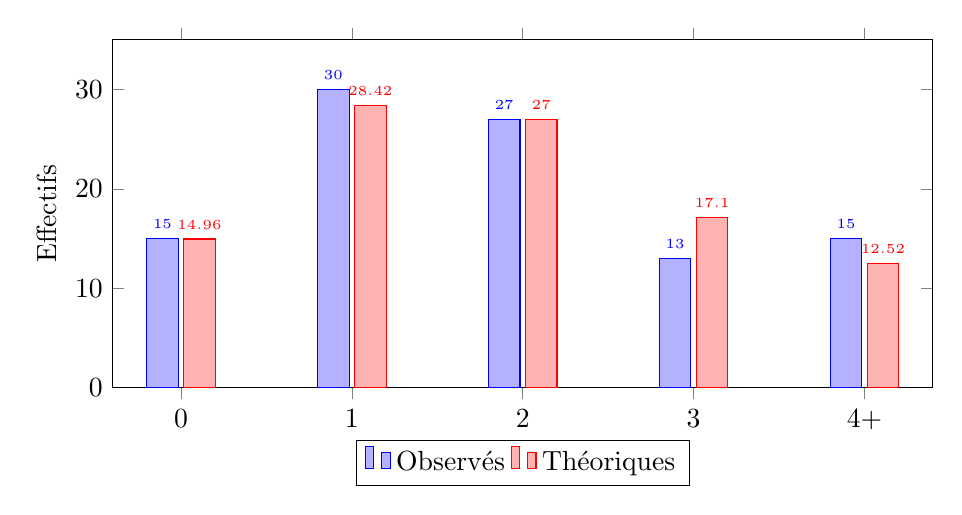
\begin{tikzpicture}
				\begin{axis}[
					ybar,
					bar width=0.4cm,
					width=12cm,
					height=6cm,
					xlabel={Nombre d'entretiens},
					ylabel={Effectifs},
					symbolic x coords={0,1,2,3,4+},
					xtick=data,
					legend style={at={(0.5,-0.15)},anchor=north,legend columns=-1},
					ymin=0,
					ymax=35,
					nodes near coords,
					every node near coord/.append style={font=\tiny}
					]
					\addplot coordinates {(0,15) (1,30) (2,27) (3,13) (4+,15)};
					\addplot coordinates {(0,14.96) (1,28.42) (2,27.00) (3,17.10) (4+,12.52)};
					\legend{Observés,Théoriques}
				\end{axis}
			\end{tikzpicture}
		\end{center}
		
		On constate visuellement que les distributions sont très proches.
		
	}
	
	\indication{
		\textbf{Utilisation d'un tableur pour les calculs :}
		
		\textbf{1. Calcul de $\lambda$ :}
		\begin{itemize}
			\item Colonne A : valeurs $k$ (0, 1, 2, 3, 4, 5, 6)
			\item Colonne B : effectifs observés $o_k$
			\item Cellule D1 : \texttt{=SOMMEPROD(A2:A8;B2:B8)/SOMME(B2:B8)} donne $\lambda = 1.90$
		\end{itemize}
		
		\textbf{2. Calcul des probabilités de Poisson :}
		\begin{itemize}
			\item Cellule C2 : \texttt{=LOI.POISSON(A2;\$D\$1;FAUX)} 
			\item Copier jusqu'à C7
			\item Cellule C8 (pour $k \geq 6$) : \texttt{=1-SOMME(C2:C7)}
		\end{itemize}
		
		\textbf{3. Calcul des effectifs théoriques :}
		\begin{itemize}
			\item Cellule D2 : \texttt{=C2*100}
			\item Copier jusqu'à D8
		\end{itemize}
		
		\textbf{4. Calcul de $\chi^2$ :}
		\begin{itemize}
			\item Regrouper les classes si nécessaire
			\item Cellule E2 : \texttt{=(B2-D2)\^{}2/D2}
			\item Copier pour chaque classe
			\item Somme : \texttt{=SOMME(E2:E6)}
		\end{itemize}
		
		\textbf{5. Valeur critique et $p$-valeur :}
		\begin{itemize}
			\item Valeur critique : \texttt{=LOI.KHIDEUX.INVERSE(0.05;3)} donne 7.815
			\item $p$-valeur : \texttt{=1-LOI.KHIDEUX(1.5613;3;VRAI)} donne 0.668
		\end{itemize}
	}
}